\chapter{Anpassning av testmetoder för småskalig utveckling av Joakim Argillander}
\section{Introduktion}
I detta avsnitt behandlas vilka frågeställningar som avhandlas, motivering och målsättning med avhandlingen.
\label{cha:joakim-introduction}

\subsection{Motivering}
\label{sec:joakim-motivation}
Att utveckla en produkt \emph{åt} en kund, till skillnad mot att utveckla åt sig själv innebär att garantier om produktens kvaliteter, såsom kravuppfyllnad, stabilitet och användbarhet måste kunna lämnas. En metod för att göra detta är mjukvarutestning. 

%This is where the studied problem is described from a general
%point of view and put in a context which makes it clear that
%it is interesting and well worth studying. The aim is to make
%the reader interested in the work and create an urge to
%continue reading.

\subsection{Målsättning}
\label{sec:joakim-aim}
Målsättningen med denna avhandling är att redogöra för- och nackdelar med agil testningsmetodik och hur man kan anpassa detta till småskalig mjukvaruutveckling. Avhandlingen syftar också till att undersöka hur man i en nystartad projektgrupp kan utveckla en testmetodik. 
%What is the underlying purpose of the thesis project?

\subsection{Frågeställningar}
\label{sec:joakim-research-questions}
%This is where the research questions are described.
%Formulate these as explicit questions, terminated with a
%question mark. A report will usually contain several different
%research questions that are somehow thematically connected.
%There are usually 2-4 questions in total.


%Examples of common types of research questions (simplified
%and generalized):
\begin{enumerate}
\item Hur kan garantier lämnas om ett mjukvarusystem av utvecklare utan tidigare erfarenhet av mjukvarutestning?
\item Hur genomförs testning så att belastningen på utvecklare blir minimal? 
\end{enumerate}

%Observe that a very specific research question almost always
%leads to a better thesis report than a general research question
%(it is simply much more difficult to make something good
%from a general research question.)

%The best way to achieve a really good and specific research
%question is to conduct a thorough literature review and get
%familiarized with related research and practice. This leads to
%ideas and terminology which allows one to express oneself
%with precision and also have something valuable to say in the
%discussion chapter. And once a detailed research question
%has been specified, it is much easier to establish a suitable
%method and thus carry out the actual thesis work much faster
%than when starting with a fairly general research question. In
%the end, it usually pays off to spend some extra time in the
%beginning working on the literature review. The thesis
%supervisor can be of assistance in deciding when the research
%question is sufficiently specific and well-grounded in related
%research.

\subsection{Avgränsningar}
\label{sec:joakim-delimitations}

Undersökningen baseras på det projektarbete som utförts som en del av kursen TDDD96 - Programutvecklingsmetodik under våren 2017.\\
\\
Verktyg och ramverk som används utgår från användandet av JavaScript-webramverket Meteor och är avgränsat till projekt baserat på nämnda ramverk.  

%This is where the main delimitations are described. For
%example, this could be that one has focused the study on a
%specific application domain or target user group. In the
%normal case, the delimitations need not be justified.

%\nocite{scigen}
%We have included Paper \ref{art:scigen}

%%%%%%%%%%%%%%%%%%%%%%%%%%%%%%%%%%%%%%%%%%%%%%%%%%%%%%%%%%%%%%%%%%%%%%
%%% Intro.tex ends here


%%% Local Variables: 
%%% mode: latex
%%% TeX-master: "demothesis"
%%% End: 


\section{Teori}
\label{cha:joakim-theory}

En metod att kvalitetssäkra mjukvara gentemot utvecklingsprojektets intressenter är mjukvarutestning. Mjukvarutestning innebär en objektiv utvärdering av en mjukvaras kvaliteter och undersökning huruvida produkten når uppställda krav på dessa.\cite{book:artoftesting} Genom en serie av olika tester, nämnda nedan, verifieras att produkten i form av mjukvaran fungerar på det sätt som utlovats i kravspecifikationen, i den användningsmiljö som den utformats att fungera i.

\begin{itemize}
\item \textbf{Enhetstester} - där individuella kodstycken testas utifrån dess ämmade funktionalitet. Dessa tester kan både vara automatiska och manuella, och testar det som kan anses vara en mjukvaras minsta testbara beståndsdel. Ingenjörssammanslutningen IEEE värderar både automatiska och manuella enhetstester likvärdigt. Vid testdriven utveckling konstrueras enhetstester först för hela funktionaliteten. Naturligt så misslyckas alla dessa tester initialt för att sedan inkrementellt lyckas vartefter utvecklingen fortskrider. Enhetstestet kan ses som ett strikt kontrakt som koden måste uppfylla, och bidrar genom detta till självdokumentation av källkoden.\cite{ieee1008}
\item \textbf{Integrationstester} - testning av sammansättning och integration av olika kodmoduler, vilka kan ses som de byggblock som utgör det kompletta systemet. Syftet är att undersöka att olika subsystem fungerar tillsammans med varandra i större aggregationer. Detta säkerställer att gränssnitten mellan moduler fungerar och bildar ett enhetligt system eller subsystem, beroende på abstraktionsnivå. Denna typ av testning görs vanligtvis efter enhetstester och funktionstester utförts.\cite{integration_testing}
\item \textbf{Funktionstester} - syftar till att testa en viss funktionalitet i ett mjukvarusystem. Med detta menas att varje utvecklad funktionalitet utvärderas och testas. Enligt ingenjörssammanslutningen IEEE rekommenderas inte att en given funktionalitet inte också testas av samma utvecklare som bidragit till att utveckla den. Detta för att kunna garantera ett objektivt testningsförfarande. 
\item \textbf{Användbarhetstest} - används för att utvärdera systemets tillsammans med dess tänkta användare. Denna typ av testning är ovärdelig för att få information om hur systemet fungerar i dess tänkta användningsmiljö. Vanligtvis låter man slutanvändare använda mjukvarusystemet genom scenarier och situationer där användaren löser ett problem och observatörer noterar om användarens interaktionssteg motsvarar de förväntade. Utifrån detta utvärderas systemets intuitivitet, användarvänlighet och användbarhet. 
\item \textbf{Regressionstest} - är en iterativ typ av test som används för att säkerställa att tidigare utvecklad kod och funktionalitet fortfarande fungerar. Denna typ av testning sker med jämna mellanrum och visar på om en funktionalitet som implementerats och klarat både enhetstest och funktionstest resulterar i att hela bygget havererar efter att den givna funktioanliteten implementerats.\cite{integration_testing}
\item \textbf{Installationstest} - testar huruvida systemet kan installeras, avinstalleras, och uppgraderas hos slutkunden. Detta kan vara en del av acceptanstestning och involverar testning av proceduerer för installation på slutkunds plattform.
\item \textbf{Acceptanstest} - testar om systemet uppfyller kravspecifikationen. Utförs ibland tillsammans med kund.
\end{itemize}
\ \\
Utöver de nämnda typer av test så finns det ett oräknerligt antal andra testtyper som alla betraktar olika mjukvarukvaliteter och ämmar till att testa dessa på ett objektivt, vetenskapligt sätt. Olika projekt använder sig av olika metoder för att genomföra mjukvarutestningen, då det finns praktiskt taget oändligt med kvaliteter att utvärdera. \\
\\
För att konkretisera testningsförfarandet formuleras ofta så kallade testfall som beskriver vad som testas, och det förväntade utfallet, samt de steg som testpersonen, eller ett automatiserat testramverk, ska utför för att utföra testet. I kapitlet \emph{Metod} behandlas hur testning kan utföras i ett småskaligt mjukvaruprojekt.

\subsection{Arbetsflöde}
För att det ska vara meningsfullt att diskutera testmetoder måste ett arbetsflöde defineras. Det arbetsflöde som använts är ett så kallat feature-branch-flöde där varje funktionalitet i en egen utvecklingsgren, avgrenad från den källkod som finns i huvudgrenen, benämnt \textit{development} i figur \ref{fig:git_workflow}.\cite{website:atlassian_git} Då kan funktionaliteten utvecklas parallellt i isolation från resterande utvecklingsarbete och integreras med huvudgrenen. Ur testhänsyn finns två intressanta tillfällen då officiell testning utförs. Innan utvecklingsgrenen ska integreras med huvudgrenen utförs enhetstestning, funktionstestning för att verifiera att funktionaliteten fungerar i isolation. När detta kan konstateras integreras huvudgrenen in i utvecklingsgrenen, och regressionstest utförs. Detta gör för att verifera att huvudgrenen fortfarande fungerar med den nya integrerade funktioanliteten och att ingen tidigare utvecklad funktionalitet har upphört att fungera i samband med sammanfogningen. Efter detta återintegreras utvecklingsgrenen (som nu innehåller huvudgrenens innehåll) med huvudgrenen.

\begin{figure}[h]
  \centering
  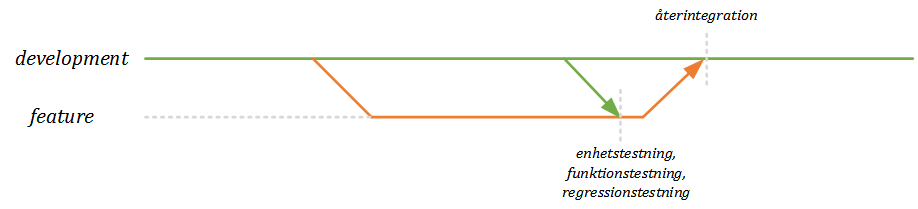
\includegraphics[scale=1]{git_workflow}
  \caption{Illustration över ett tänkt arbetsflöde}
  \label{fig:git_workflow}
\end{figure}
%The main purpose of this chapter is to make it obvious for
%the reader that the report authors have made an effort to read
%up on related research and other information of relevance for
%the research questions. It is a question of trust. Can I as a
%reader rely on what the authors are saying? If it is obvious
%that the authors know the topic area well and clearly present
%their lessons learned, it raises the perceived quality of the
%entire report.

%After having read the theory chapter it shall be obvious for
%the reader that the research questions are both well
%formulated and relevant.

%The chapter must contain theory of use for the intended
%study, both in terms of technique and method. If a final thesis
%project is about the development of a new search engine for
%a certain application domain, the theory must bring up related
%work on search algorithms and related techniques, but also
%methods for evaluating search engines, including
%performance measures such as precision, accuracy and
%recall.

%The chapter shall be structured thematically, not per author.
%A good approach to making a review of scientific literature
%is to use \emph{Google Scholar} (which also has the useful function
%\emph{Cite}). By iterating between searching for articles and reading
%abstracts to find new terms to guide further searches, it is
%fairly straight forward to locate good and relevant
%information, such as \cite{test}.

%Having found a relevant article one can use the function for
%viewing other articles that have cited this particular article,
%and also go through the article’s own reference list. Among
%these articles on can often find other interesting articles and%
%thus proceed further.

%It can also be a good idea to consider which sources seem
%most relevant for the problem area at hand. Are there any
%special conference or journal that often occurs one can search
%in more detail in lists of published articles from these venues
%in particular. One can also search for the web sites of
%important authors and investigate what they have published
%in general.

%This chapter is called either \emph{Theory, Related Work}, or
%\emph{Related Research}. Check with your supervisor.%


\section{Metod}
\label{cha:joakim-method}
Genom att iterativt arbeta fram en strategi för mjukvarutestning baserat på IEEE-standarder \emph{IEEE std 1008} samt \emph{ISO25010} under projektets gång har resultatet tagits fram.\cite{ieee1008}\cite{iso25010} Då projektarbetet genomgick flertalet iterationer gavs möjligheten att utveckla testarbetet till nästkommande iteration. Även vid skapande av testrapporter gavs tid för eftertanke och planering av nästkommande iterations testning, där det nuvarande testningsförfarandet utvärderades och sedemera även reviderades.

\section{Resultat}
\label{cha:joakim-results}
Att genomföra testning som lämnar garantier om mjukvarans kvaliteter genom heltäckande tester kan utföras på en mängd olika sätt. Här behandlas ett alternativ, där testning behandlas likvärdigt med andra utvecklingsuppgifter, samt hur etablerade standarder och riktlinjer kan anpassas för användning i ett småskaligt agilt mjukvaruprojekt. Efterforskningarna resulterade i ett färdigt ramverk för mjukvarutestning baserat på ISO/IEEE-standarder som inte kräver kännedom om dessa standarder, utan är färdigt applicerbart på ett godtyckligt valt mjukvaruutvecklingsprojekt.

\subsection{Enhetstest}
Enhetstester utförs med hjälp av enhetstestramverket Mocha, tillsammans med biblioteket Chai som ger tillgång till funktionalitet för att validera huruvida funktioners in-/utdata motsvarar förväntade värden.\cite{website:mocha}\cite{website:chai} Varje utvecklare är ansvarig för att belägga den incheckade koden med enhetstester. 

\subsection{Funktionstest}
Till varje utvecklad funktionalitet, buggfix eller kodunderhåll formuleras ett testfall. Detta testfall formuleras enligt överenskommet format för att undvika tvetydigheter som kan uppstå mellan testare och utvecklare. Testfallet utförs av en utvecklare som valts att testa den givna utvecklingsuppgiften, där enhetstest ingår i standardformuleringen för testfall. 

\subsubsection{Utformning av testfall}
Testfallen formuleras utifrån utvecklingsuppgiften, och hör samman som en bilaga till den. Under projektarbetets gång användes Trello, ett webbaserat projekthanteringssystem där varje utvecklingsuppgift gavs ett \emph{utvecklingskort} och varje testuppgift bifogades till utvecklingskortet.\cite{website:trello}

\subsection{Regressionstest}
Utvecklingsarbetet regressionstestas genom att tidigare utvecklingsuppgifters testfall utförs. Då verifieras att ingen tidigare utvecklad funktionalitet har brutits. Resultatet av regressionstestet förs in i en testlogg för att göra det möjligt att följa upp systemets status under utvecklingens gång. 

\subsection{Acceptanstest}
Ett internt acceptanstest utförs med marginal innan acceptanstest med kund. Tid planeras mellan de båda acceptanstesterna för att eventuella felaktigheter, både i kravuppfyllnad och funktionalitet, ska hinna åtgärdas innan acceptanstest med kund. Återigen planeras för att eventuella felaktigheter kan uppstå under acceptanstest med kund, sådant att dessa kan åtgärdas innan leverans. Acceptanstestet genomförs genom att presentera kravspecifikationen, samt vad som utvecklats i systemet för att uppnå dessa krav. Under acceptanstestet med kund bör också ett användbarhetstest att utföras.\cite{arvolaboken}.
%This chapter presents the results. Note that the results are presented
%factually, striving for objectivity as far as possible.  The results
%shall not be analyzed, discussed or evaluated.  This is left for the
%discussion chapter.

%In case results are presented from a process (e.g. an implementation
%process), the main decisions made during the process must be clearly
%presented and justified. Normally, alternative attempts, etc, have
%already been described in the theory chapter, making it possible to
%refer to it as part of the justification.

\section{Diskussion}
\label{cha:joakim-discussion}
Metoden för testning som utvecklats under projektets gång har visat sig vara en anpassning av agila testmetoder och andra standardmetoder som fungerat väl för ett mindre utvecklingsprojekt. Metoderna för de olika typerna av testning är enkla och belastar inte utvecklarna nämnvärt, utan planeras som en naturlig del av utvecklingen. Trots att mycket talar för att den föreslagna testningen bör att genomföra med utvecklare som inte tidigare använt sig av mjukvarutestning i utvecklingen så föranligger en risk med omfattande testmoment. Så länge utvecklare inte ser någon vinning i att kvalitetssäkra produkten genom mjukvarutestning så blir även den bästa testmetodiken verkningslös. Under projektets gång upplevdes det ibland att testningen förbisågs och bortprioriterades. Här kan föreslås att använda enskilda testare eller deltidsutvecklare med deltidsansvar för testning för att både avlasta utvecklare men ändå lämna testbara garantier. Ett annat alternativ är att skifta större fokus till regressionstestning och att istället för att utvärdera varje utvecklad funktionalitet direkt så genomförs rigorösa regressionstester veckovis. Detta eftersom utvecklingsuppgifterna ibland kan vara små, i synnerhet när det handlar om underhåll av systemet, varvid testmomentet kan ta större tid i anspråk än att lösa uppgiften. Detta hade avhjälpts av att endast funktionstesta större moduler och inte enskilda utvecklingsuppgifter, vilket är ytterligare ett alternativ. \\
\\
Den agila arbetssättet som användes under projektets gång tillät testmetoderna att iterativt utvecklas och anpassas till något som fungerade för den givna projektgruppen med dess förutsättningar.
Arbetsgången för att utveckla testprocessen är anpassad utifrån utvecklare som saknar tidigare erfarenhet av organiserad mjukvarutestning och innehåller därför många utvärderingsmoment. Utveckling av testmetoder har också setts som ett pågående arbete öppet för förbättringar även under iterationer. Initialt användes användes \emph{The Art of Software Testing} som utgångspunkt, vilken gav ett stort stöd i att konkretisera vilka olika typer av testning som kan tänkas nödvändiga i det utförda projektet.\cite{book:artoftesting}\\
\\
Ett annat angreppssätt hade varit att låta ett designerat testpar eller en testare utföra all mjukvarutestning. Det hade lett till att testaren får en övergripande bild av systemets status, vet var testerna fallerar och kan se vilken funktionalitet som kan påverka att någon annan del av mjukvaran havererar. Däremot hade detta lett till att antalet utvecklare minskat, och större utvecklingsbörda hade lagts på återstående utvecklare.
%This is where the applied method is discussed and criticized.
%Taking a self-critical stance to the method used is an
%important part of the scientific approach.

%A study is rarely perfect. There are almost always things one
%could have done differently if the study could be repeated or
%with extra resources. Go through the most important
%limitations with your method and discuss potential
%consequences for the results. Connect back to the method
%theory presented in the theory chapter. Refer explicitly to
%relevant sources.

%The discussion shall also demonstrate an awareness of methodological
%concepts such as replicability, reliability, and validity. The concept
%of replicability has already been discussed in the Method chapter
%(\ref{cha:method}). Reliability is a term for whether one can expect
%to get the same results if a study is repeated with the same method. A
%study with a high degree of reliability has a large probability of
%leading to similar results if repeated. The concept of validity is,
%somewhat simplified, concerned with whether a performed measurement
%actually measures what one thinks is being measured. A study with a
%high degree of validity thus has a high level of credibility. A
%discussion of these concepts must be transferred to the actual context
%of the study.

%The method discussion shall also contain a paragraph of
%source criticism. This is where the authors’ point of view on
%the use and selection of sources is described.

%In certain contexts it may be the case that the most relevant
%information for the study is not to be found in scientific
%literature but rather with individual software developers and
%open source projects. It must then be clearly stated that
%efforts have been made to gain access to this information,
%e.g. by direct communication with developers and/or through
%discussion forums, etc. Efforts must also be made to indicate
%the lack of relevant research literature. The precise manner
%of such investigations must be clearly specified in a method
%section. The paragraph on source criticism must critically
%discuss these approaches.

%Usually however, there are always relevant related research.
%If not about the actual research questions, there is certainly
%important information about the domain under study.

%There must be a section discussing ethical and societal
%aspects related to the work. This is important for the authors
%to demonstrate a professional maturity and also for achieving
%the education goals. If the work, for some reason, completely
%lacks a connection to ethical or societal aspects this must be
%explicitly stated and justified in the section Delimitations in
%the introduction chapter.

%In the discussion chapter, one must explicitly refer to sources
%relevant to the discussion.
\section{Slutsatser}
\label{cha:joakim-conclusion}
Därför föreslås att denna metod för testning kan vara lämplig att använda även i utbildningssyften, men för att använda den praktiskt krävs en förståelse för vinningen av att kontinuerligt utvärdera produktens kravuppfyllelse, funktionalitet och stabilitet. Detta motiveras genom att ha utvärderat användandet under projektets gång där testningen varit så pass täckande att garantier kan lämnas om kravuppfyllnad och genom att studera hur testloggar överensstämmer med kod som har återintegrerats in i projektets huvudgren. \\
\\
Att kontinuerligt dokumentera testning har visat sig viktigt och är också någonting som anses nödvändigt både för att upprätthålla en spårbarhet i arbetsflödet, men även för att kunna utvärdera och utveckla den testning som utförs. Med detta menas att kontinuerliga testrapporter med utvecklingsmöjligheter bör föras samt diskuteras med de berörda utvecklarna för att ha möjlighet att lyfta sådant som kan riskera att mjukvarutestningen förbises och bortprioriteras.
%This chapter contains a summarization of the purpose and the research
%questions. To what extent has the aim been achieved, and what are the
%answers to the research questions?

%The consequences for the target audience (and possibly for researchers
%and practitioners) must also be described. There should be a section
%on future work where ideas for continued work are described. If the
%conclusion chapter contains such a section, the ideas described
%therein must be concrete and well thought through.
